	\chapter{Kravspecifikation}
	Dette afsnit indeholder systembeskrivelse, en central use case og de første tanker omkring design og GUI. \\
	
		\section{Systembeskrivelse}
		Der ønskes lavet en applikation som får folk til at lege mere med farveskift af lyset på deres Philips Hue pærer.
		Applikationen skal kunne skifte lyset instant, gemme temaer man kan sætte i gang på givende tidspunkter, måske hvis en speciel playliste bliver sat på. Man skal kunne bruge applikationen til at betjene flere forskellige pærer.
		Der vil blive udviklet en applikation som snakker op til et API, som er udstedet af et andet firma, for at se at dette faktisk er en reel arbejdsmodel man kan bruge i hverdagen.
		Dette sker ved at der i applikationen skal snakkes op til Philips Hue API for at kunne tilgå pærerne.
			
		\subsection{Use Cases}
		Use Case 1:
		\begin{itemize}
			\item Bruger ønsker at connecte til Hue bridge første gang
			\item Bruger starter Shine My Room
			\item Bruger bliver bedt om trykke på "Push to link" knappen på bridgen, for at identifisere den
			\item Shine My Rooms status bar opdateres efter connection
		\end{itemize}
		
		Use Case 2:
		\begin{itemize}
			\item Bruger kommer hjem
			\item Bruger tænder sin Philips Hue pærer
			\item Bruger ændre lysstyrken på pæren
			\item Bruger slukker pæren
		\end{itemize}
	
		Use Case 3:
		\begin{itemize}
			\item Bruger ønsker at tilføje et rum
			\item Bruger navigere over i Edit / Add tabben
			\item Bruger trykker på Add Room knappen
			\item Bruger giver rummet et navn
			\item Bruger vælger hvilke pære rummet skal indeholde
			\item Bruger være gem bliver navigeret tilbage til forrige activity med gemt rum [Extention 1]
		\end{itemize}
		[Extention 1]: Bruger vælger cancel og bliver navigeret tilbage til forrige activity uden gemt rum
		\newpage
		
		Use Case 4:
		\begin{itemize}
			\item Bruger ønsker at aktivere geofencing
			\item Bruger navigere over i geofencing tabben
			\item Bruger aktivere geofencing
			\item Bruger forlader hjemmet
			\item Pærene slukker når han er udenfor geofencing loaction
		\end{itemize}
		
		\subsection{Ikke-funktionelle krav}
		Nedenfor ses de ikke funktionelle krav til applikationen
		\begin{itemize}
			\item Mindst to Activities
			\item Bruge Intents til at sende data mellem komponenter
			\item Persisting data gennem SharedPrefrences eller SQLite
			\item En anden form for kommunikation gemmen internet, Bluetooth eller WIFI
			\item Mindst en service
			\item Bruge Asynchronous processing
			\item Bruge nødvendig resource externalization
			\item Understøtte layouts til mindst to forskellige skærm størrelser
			\item Understøtte mindst to sporg (Dansk og Engelsk)
		\end{itemize}
				
		\section{Designovervejelser}
		Billedet herunder beskriver vores første design tanker til applikationen
		\begin{figure}[H]
			\centering
			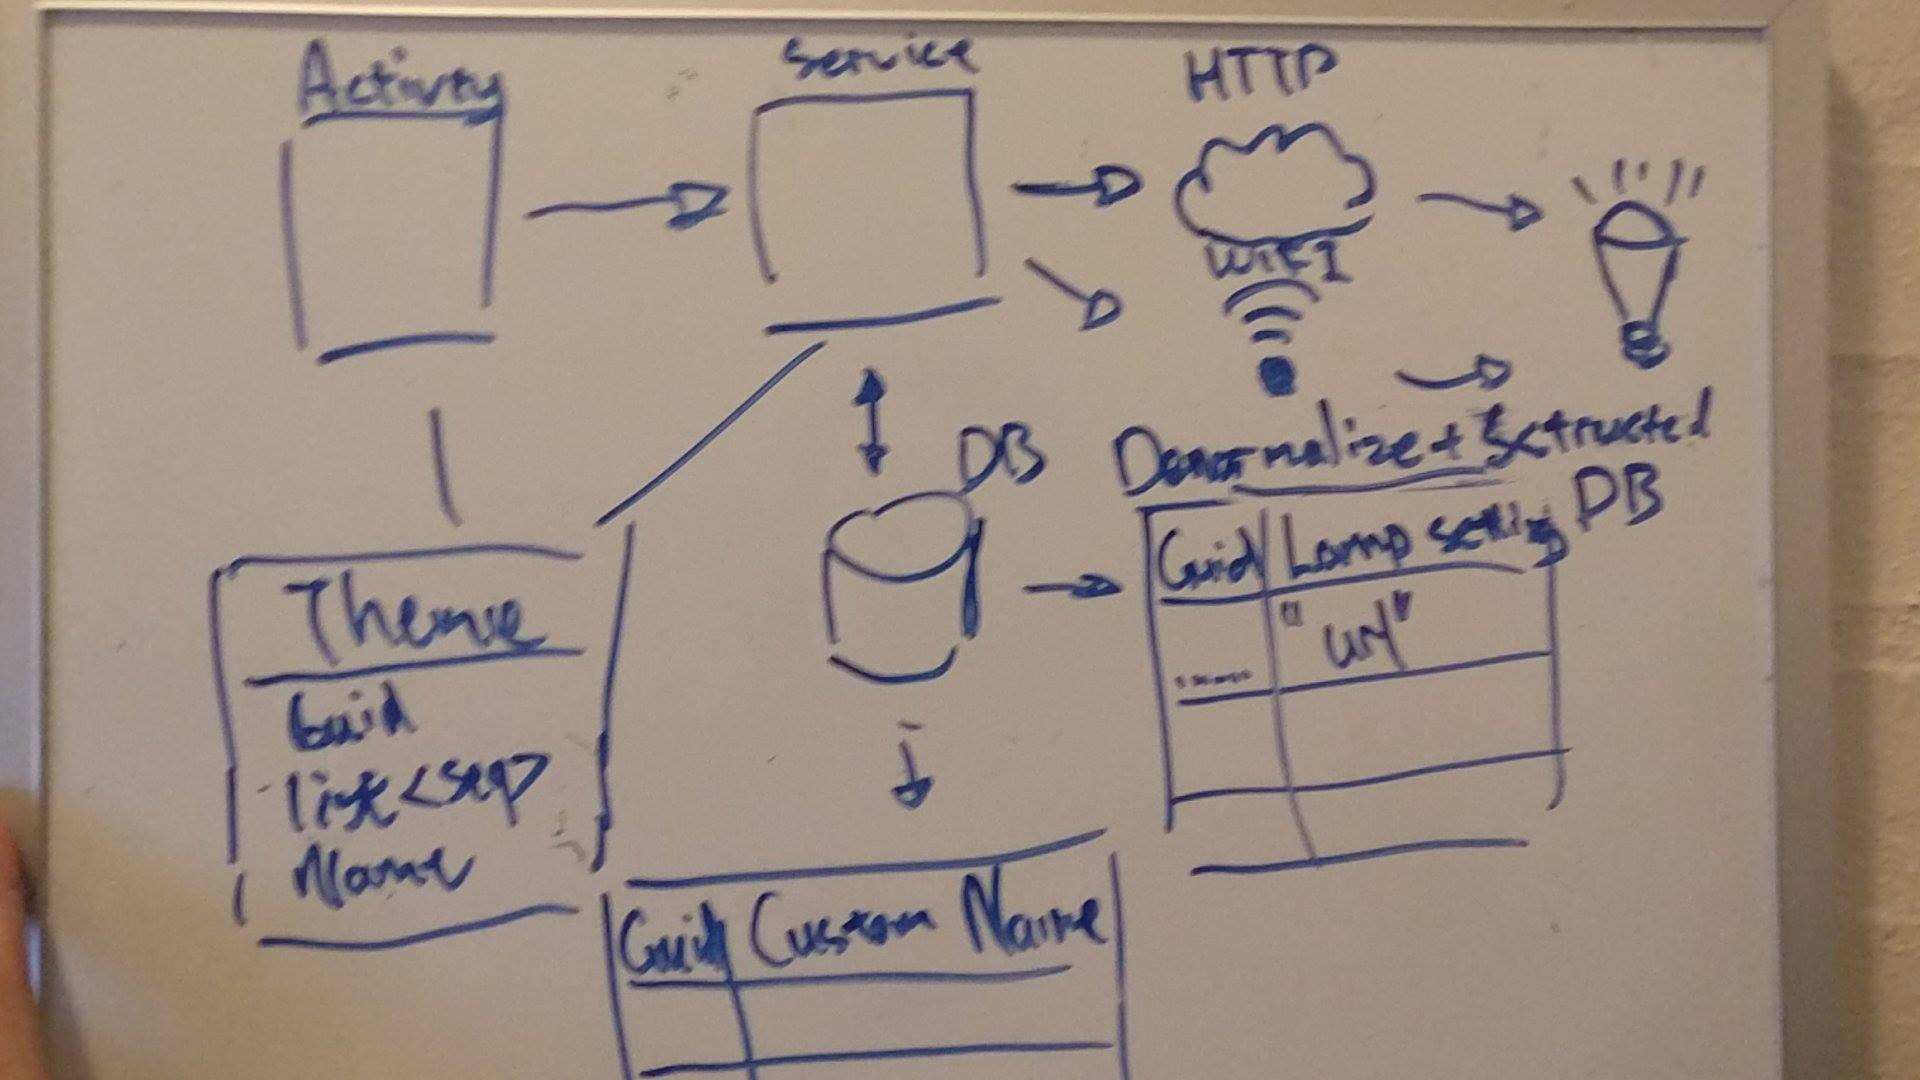
\includegraphics[width=0.9\linewidth]{Kravspecifikation/Designovervejelser}
			\caption{Oversigt over systemet}
			\label{fig:Designovervejelser}
		\end{figure}
		\newpage	
				
		\section{Første GUI udkast}
		Billedet herunder beskriver vores første GUI tanker til applikationen
		\begin{figure}[H]
			\centering
			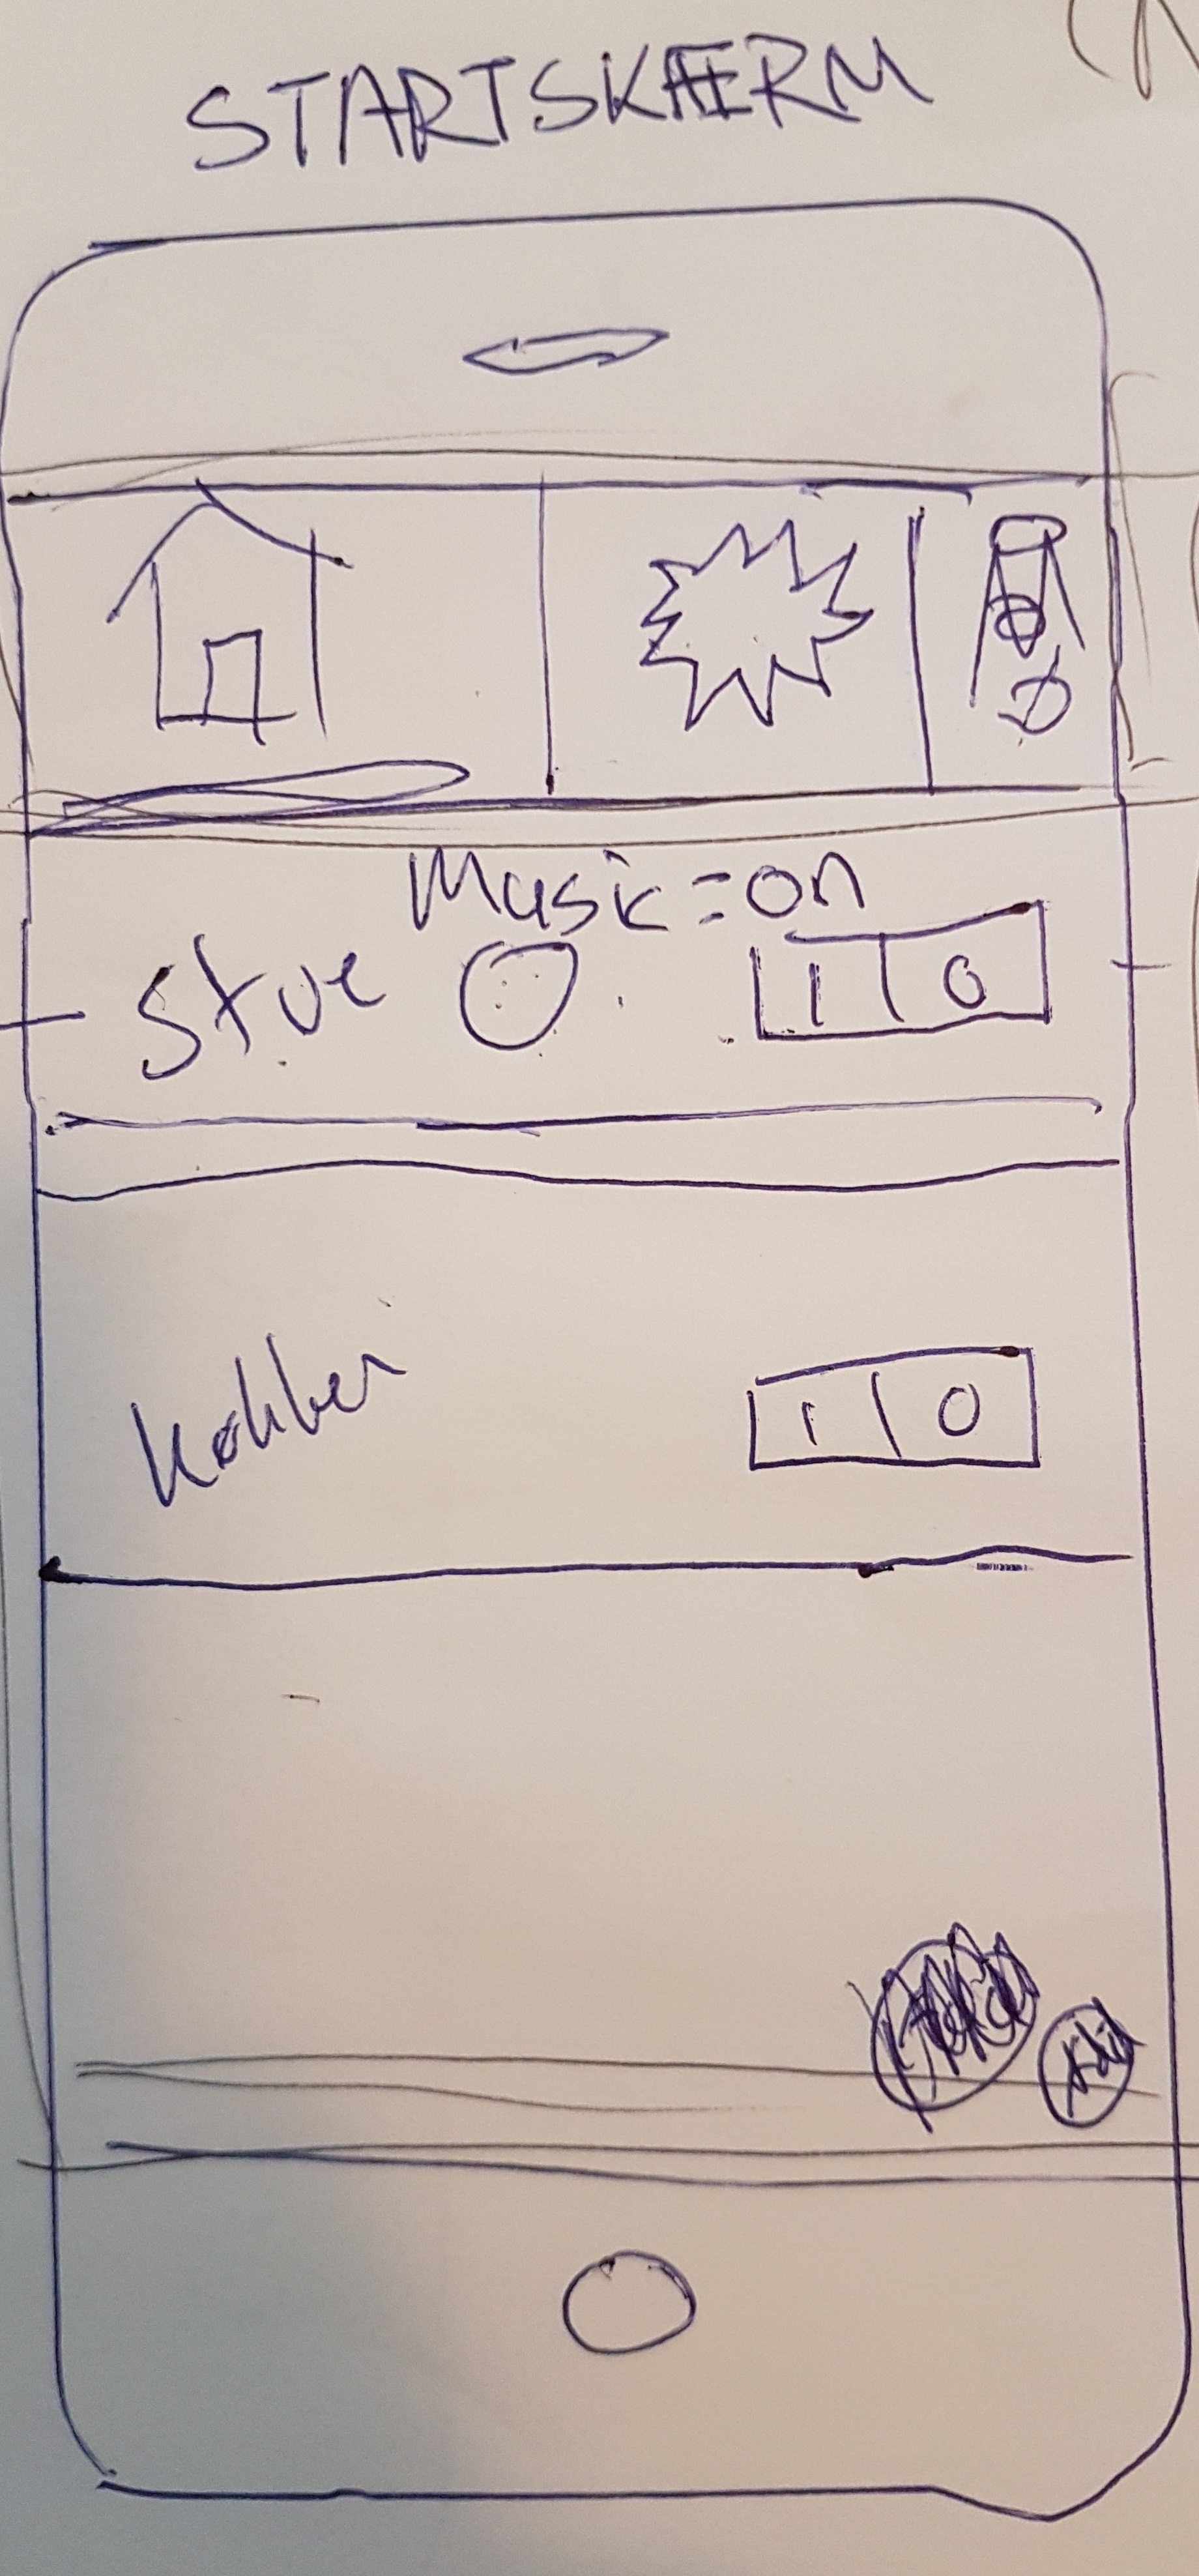
\includegraphics[width=0.6\linewidth, height=1\linewidth]{Kravspecifikation/GUI}
			\caption{GUI udkast}
			\label{fig:GUI udkast}
		\end{figure}
	
		\section{Work plan}
		\textbf{Ao Li} \\
		Har haft hovedfokus på Activities, Services og connection til Hue API
		
		\textbf{Morten Sand Knudsen} \\
		Har hovedfokus på Activities, Fragments og Adapter 
		
		Der blev i starten arbejdet sammen, men efterfølgende blev der paralleliseret med opgaver. 
		
	